\chapter{Kalgan}
Zhangjiakou (Kalgan) is a 
water-scarce city was historically the chief northern gate in the Great Wall 
to China for Europeans travelling along the Tea Road (such as Ivan Petlin (1619)[1] 
or Nicolae Milescu).

\begin{figure}[htbp]
\centering
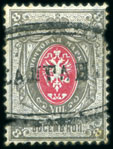
\includegraphics[width=.30\textwidth]{../russian-post-offices-in-china/10046.jpg}
\caption{
10046	KALGAN: 1875 8k Arms with dateless straight-line cancel in double 
oval (T\&S type 1), tiny thin at upper left otherwise fine and very rare.
Provenance: Ex Pappadopoulos, Blomfield and Torrey.
\euro 4,000.00 
}  
\end{figure}

In August 1211, there raised the Badger's Mount Campaign, Genghis Khan 90,000 
strong force destroyed the 450,000 strong Jin Dynasty army.
In the 19th century, the town was the seat of a very extensive transit trade. 
In early autumn long lines of camels would come in from all quarters for the conveyance of the tea chests from Zhangjiakou, the Kalgan, to Kyakhta; and each caravan usually made three journeys in the winter. 
Some Russian merchants had permanent residences and warehouses just outside the gate.
In October 1909, Kalgan was connected by railway with Peking. 
The 1911 Encyclop\ae dia Britannica noted that, in Kalgan, 
"the ordinary houses have an unusual appearance, from the fact 
that they are mostly roofed with earth and become covered with green-sward" 
and that "on the way to Peking the road passes over a beautiful bridge of 
seven arches, ornamented with marble figures of animals".

In 1937 the Japanese occupied the region and made Kalgan the capital of the 
autonomous Cha-nan (South Chahar) Province. The Federated Mengjiang 
Commission was set up to supervise the economic affairs, banking, 
communications, and industry of Japanese-occupied Inner Mongolia (Mengjiang).

In the early 1960s at the height of Sino-Soviet tensions, Zhangjiakou 
was considered one of the most important cities in China for military 
strategy reasons. Zhangjiakou was aptly nicknamed, "Beijing's Northern Door", 
because whoever controlled Zhangjiakou was in a good position to either attack 
(in the case of the Soviets) or defend (in the case of the Chinese) Beijing.

   

\begin{figure}[htbp]
\centering
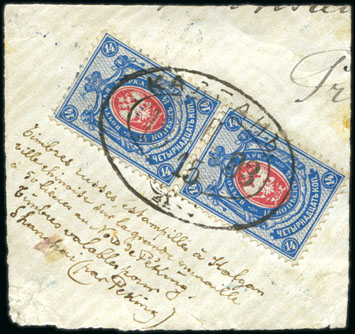
\includegraphics[width=.60\textwidth]{../russian-post-offices-in-china/10047.jpg}
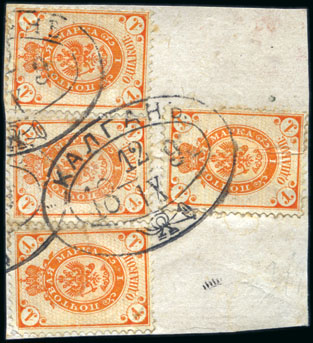
\includegraphics[width=.60\textwidth]{../russian-post-offices-in-china/10047-1.jpg}
\caption{
10047	KALGAN: Selection of stamps with Kalgan cancels incl. piece 
with four 1k tied by T\&S type 2 oval ds, piece with 1k pair tied by 
type 2 oval ds (unrecorded subtype with month above day), 7k with 
blue type 2 oval ds (unrecorded subtype with month in Arabic numerals), 
2k with type 2 oval ds (unrecorded subtype with right year digits missing 
and date above month) and a 1R and a 50k with type 2 oval ds 
(unrecorded subtype with right year digits missing and month above date), 
some minor faults
\euro 600.00
}  
\end{figure} 

\begin{figure}[htbp]
\centering
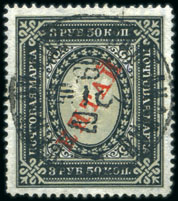
\includegraphics[width=.30\textwidth]{../russian-post-offices-in-china/10048-1.jpg}
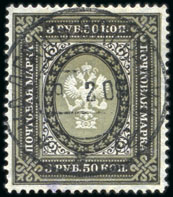
\includegraphics[width=.30\textwidth]{../russian-post-offices-in-china/10048-2.jpg}
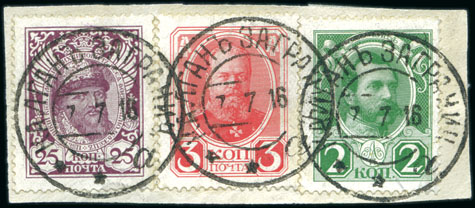
\includegraphics[width=.90\textwidth]{../russian-post-offices-in-china/10048.jpg}
\caption{
10048	KALGAN: Selection of used stamps incl. 7k with forged T\&S type 2 oval ds, 
type 2 oval ds on piece with 1k and 3k (2) and in red on 2k (only known Kalgan 
cancel in red), type 3 cds on 7k and "KITAI" 1R and 3R50, and type 5 on piece 
with Romanov 2k, 3k and 25k, on piece with Romanov 7k, 14k and 15k, and single 
3R50, some minor faults
\euro 400.00
}  
\end{figure} 

\begin{figure}[htbp]
\centering
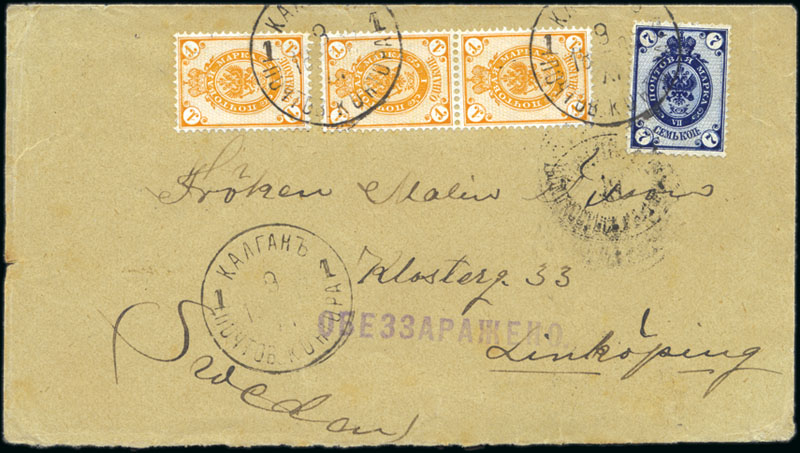
\includegraphics[width=.95\textwidth]{../russian-post-offices-in-china/10049.jpg}
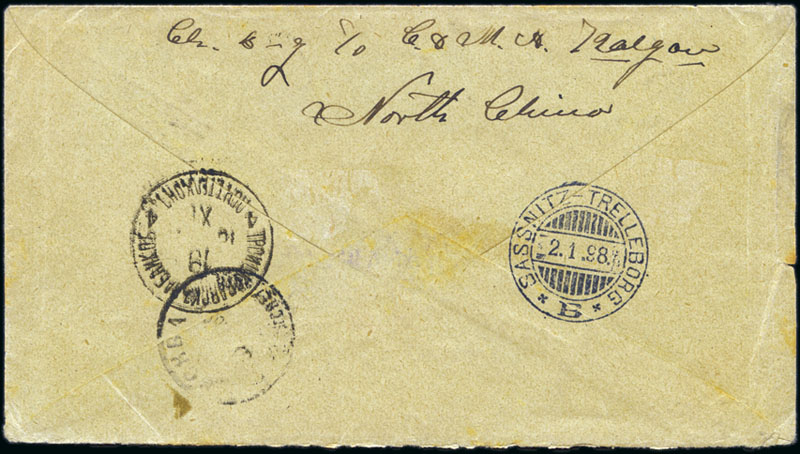
\includegraphics[width=.95\textwidth]{../russian-post-offices-in-china/10049-1.jpg}
\caption{
10049		ZoomKALGAN: 1897 Cover to Sweden with Arms 1k (3) and 7k tied
by single circle Kalgan 9.11.97 cds (not recorded by T\&S, Casey type 4), 
sent via Troitskosavsk where it was struck with violet disinfection mark, 
one of only two known covers bearing this cancel.
Note: See the "British Journal of Russian Philately" no.46 (1971) p.6, 
and 94/65 (2006) p.13
\euro 20,000.00 
}  
\end{figure}

\begin{figure}[htbp]
\centering
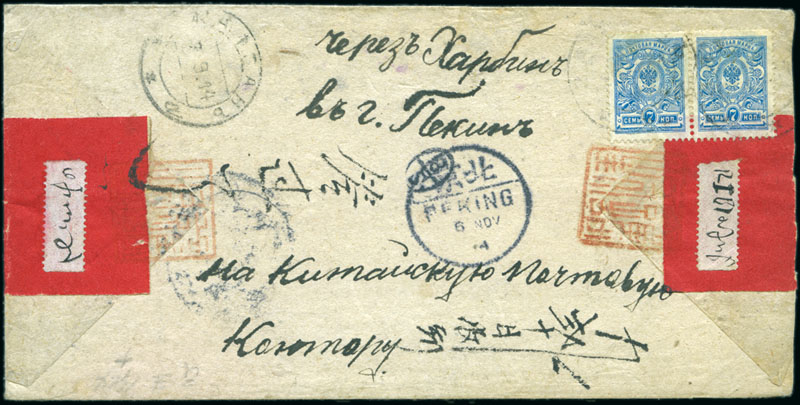
\includegraphics[width=.95\textwidth]{../russian-post-offices-in-china/10050.jpg}
\caption{
10050	KALGAN: 1914 Native cover to Peking via Harbin, Manchuria, with 
ordinary Russian 7k pair tied by Kalgan 7.9.14 cds (T\&S type 4, Casey type 7), 
received at the Russian and Chinese P.O. at Peking after incredible route across 
Mongolia, Siberia and Manchuria, very rare as no other covers are recorded with 
this Kalgan cancellation
Note: Illustrated BJRP 94/95, p.16
\euro 4,000.00
}  
\end{figure} 

\begin{figure}[htbp]
\centering
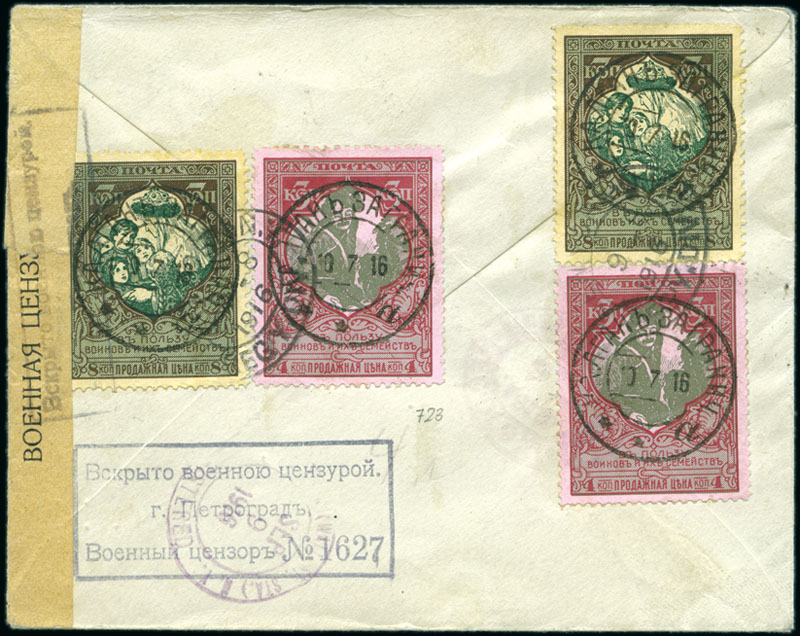
\includegraphics[width=.95\textwidth]{../russian-post-offices-in-china/10051.jpg}
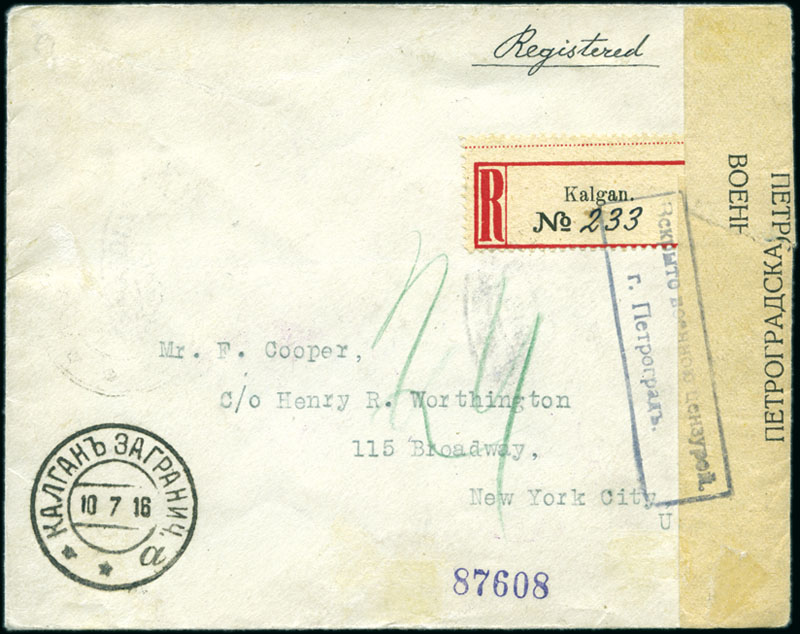
\includegraphics[width=.95\textwidth]{../russian-post-offices-in-china/10051-1.jpg}
\caption{
10051 KALGAN: 1916 Cover registered to the USA, franked on the reverse with 
War Charity 3k (2) and 7k (2) paying the 10k foreign rate plus reg'n fee, 
tied by Kalgan 10.7.16 cds (T\&S type 5, Casey type 6), opened and resealed 
by censor at Petrograd, reg'd label on obverse in English, a rare use of 
the War Charity issue.
Note: Illustrated BJRP 94/95, p.17
\euro 2,000.00 
}  
\end{figure} 




















                                                